%%%%%%%%%%%%%%%%%%%%%%%%%%%%%%%%%%%%%%%%%%%%%%%%%%%
%
%  New template code for TAMU Theses and Dissertations starting Fall 2016.
%
%
%  Author: Sean Zachary Roberson
%  Version 3.17.09
%  Last Updated: 9/21/2017
%
%%%%%%%%%%%%%%%%%%%%%%%%%%%%%%%%%%%%%%%%%%%%%%%%%%%
%%%%%%%%%%%%%%%%%%%%%%%%%%%%%%%%%%%%%%%%%%%%%%%%%%%%%%%%%%%%%%%%%%%%%%
%%                           TIME TO SOLUTION ESTIMATOR CHAPTER
%%%%%%%%%%%%%%%%%%%%%%%%%%%%%%%%%%%%%%%%%%%%%%%%%%%%%%%%%%%%%%%%%%%%%



\chapter{PARTITIONING OPTIMIZATION \label{cha:optimization}}
In Chapter \ref{cha:tts}, we have seen that we can estimate the time-to-solution for a sweep for different partitioning schemes.
We use the time-to-solution estimator as the objective function in two optimization methods.
The first optimization method utilizes scipy's optimize library, and the second method utilizes knowledge of a problem's mesh layout to assist in partition placement.
%%%%%%%%%%%%%%%%%%%%%%%%%%%%
\section{Scipy optimize}
The scipy optimize library \cite{scipy} provides many tools for optimizing an input function with local and global minimization techniques.
Our usage of the optimize library relies on the minimize function, using the basinhopping \cite{basinhoppingwales} method as the global optimizer, and the constrained Nelder-Mead method as the local optimizer.
We need a global optimization method for larger problem spaces to ensure that cut planes/lines are getting optimized over the entirety of the problem domain, rather than just moving the cut planes/lines close to our initial guess.

The black box tools of scipy optimize are too dependent on the smoothness of the function being optimized.
The time-to-solution estimator is not easily differentiable, and therefore not a smooth enough function even for the parameter spaces of a domain decomposed into 3 subsets in each dimension.
Although utilizing a tested and documented optimizer would have been ideal, it is clear that we need a method more uniquely suited for our problem.

\section{CDF Optimization}

The ``black box'' method using scipy optimize's basinhopping and constrained Nelder-Mead minimizers can function for very small parameter spaces.
However, even with modestly large parameter spaces such as the one seen in the Level 2 experiment (Fig. \ref{level2_nocut}), the time-to-solution estimator function is not smooth enough for scipy optimize to honor the constraints or bounds of the problem, leading to the time-to-solution estimator crashing.
This lead to the development of an alternative method, the CDF optimization method.

The CDF optimization method utilizes the geometrical information of the problem to attempt to find optimal cuts. This method prioritizes finding cut line locations that cut along a ``natural boundary'', and minimizing the total number of times the time-to-solution estimator needs to be run.
The time-to-solution estimator for moderately sized problems (such as the Level 2 experiment) can take up to 20 seconds to run for one set of partitions.
This rules out a brute force method of running every possible set of partitions.
Instead, we select our cut lines from the natural boundaries of the mesh.

A natural boundary is a subset boundary that coincides with the geometrical features of the mesh. In Fig.~\ref{natural_boundary_example}, we notice natural boundaries every centimeter in each dimension.
 \begin{figure}[h]
\centering
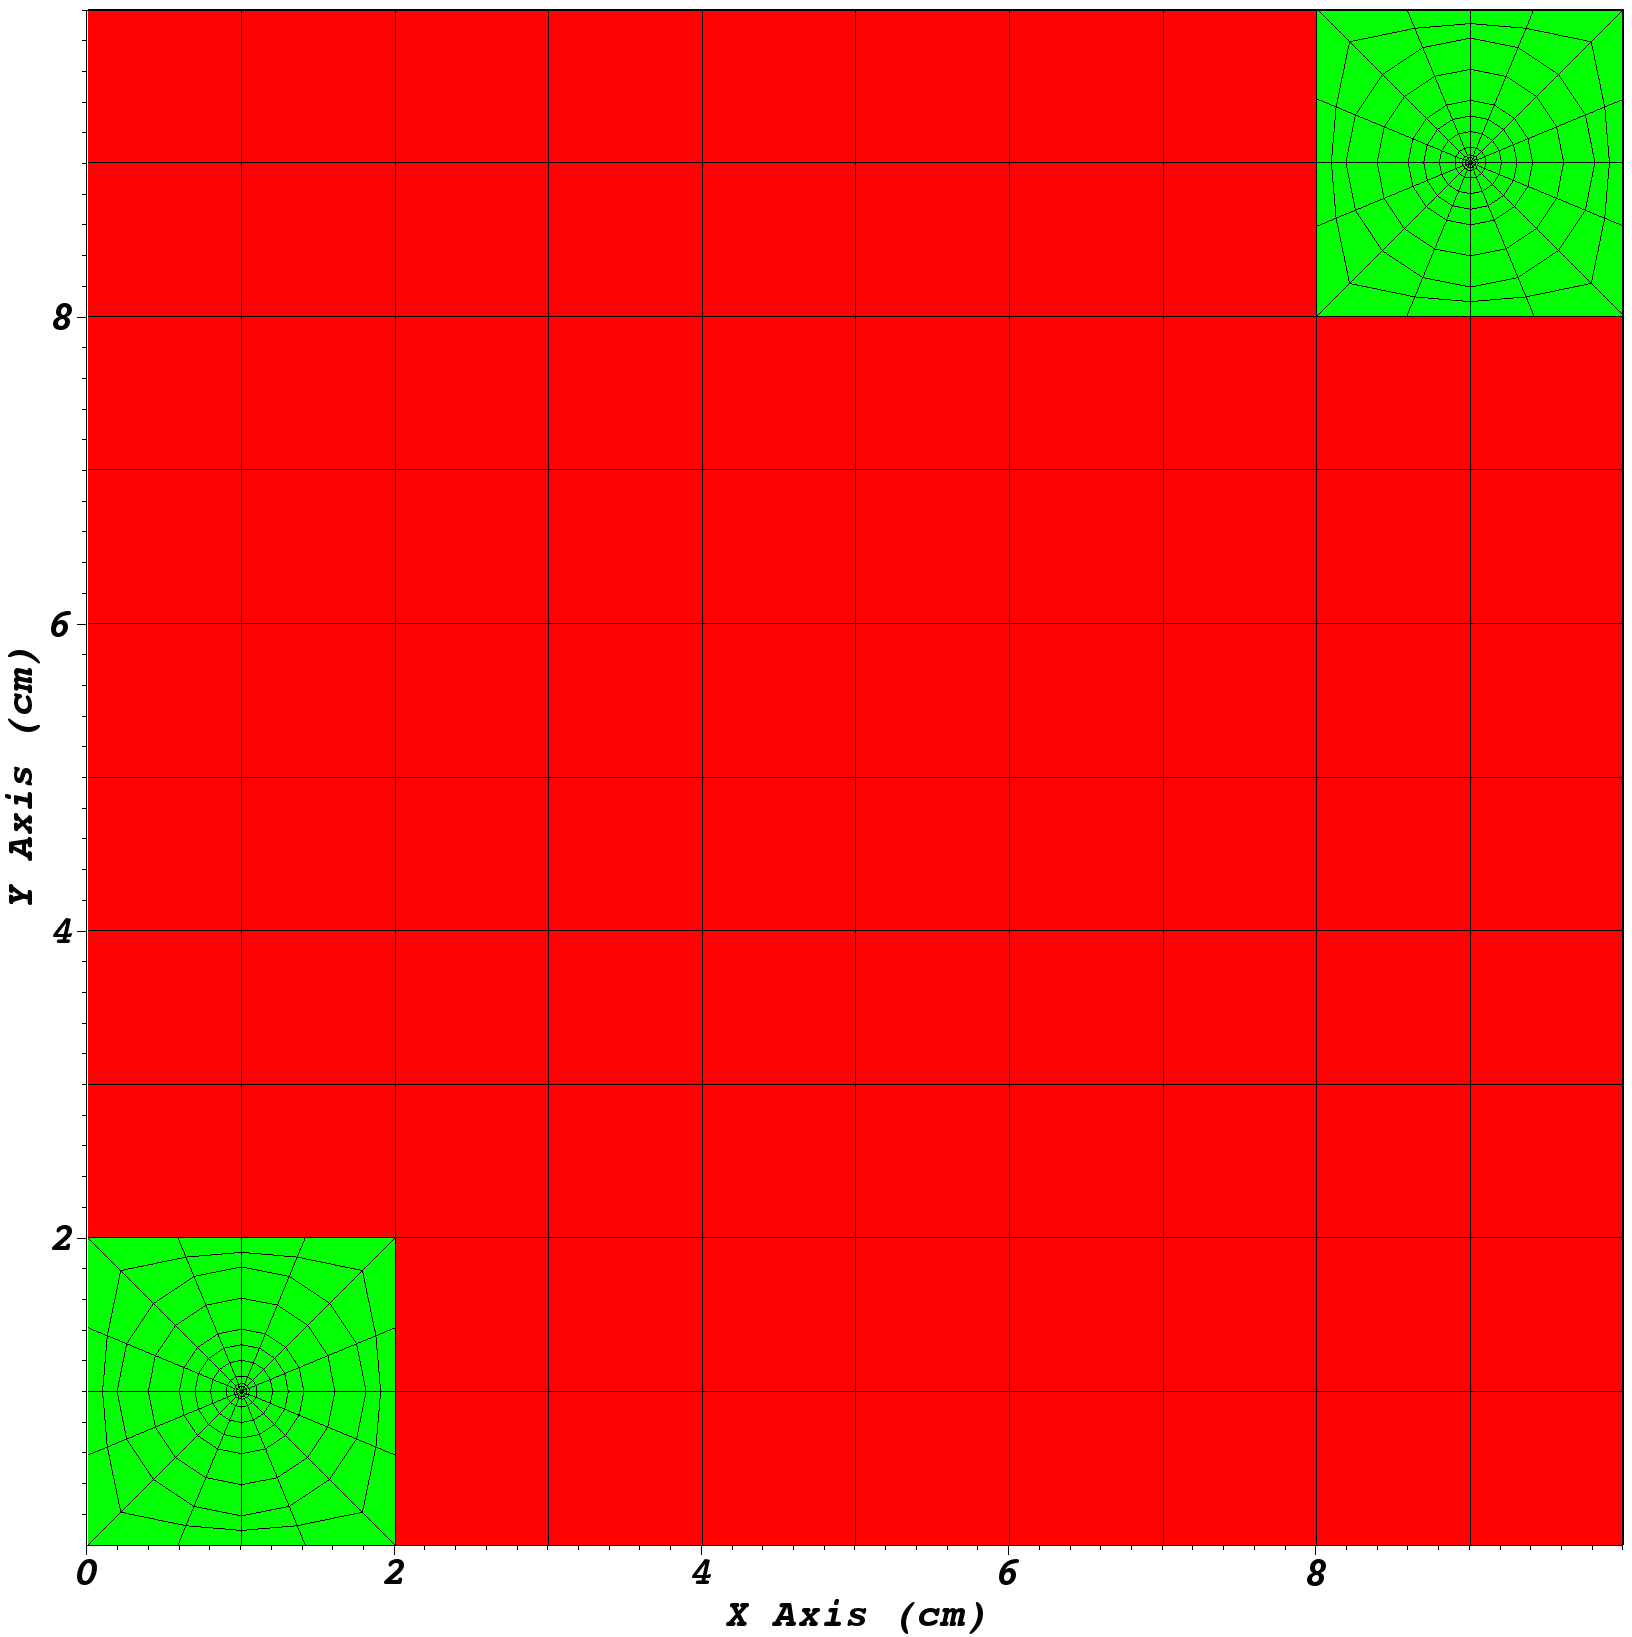
\includegraphics[scale=0.2]{../figures/spiderweb_10x10_sparse.png}
\caption{An unstructured mesh with natural boundaries at 1 cm intervals in both dimensions.}
\label{natural_boundary_example}
\end{figure}

The CDF optimization method will:
\begin{enumerate}
  \item Find the most suitable natural boundaries in the $x$ dimension,
  \item For each set of columns, find the most suitable natural boundaries in the $y$ dimension,
  \item Run all iterations of cut lines selected.
\end{enumerate}

\subsection{Finding Natural Boundaries}

In order to identify natural boundaries, we analyze the detailed cumulative distribution function (CDF) of the vertices in each dimension. The jumps in the CDF correspond to natural boundaries. Figure~\ref{vert_cdf} shows the x-vertex CDF of the mesh in Fig.~\ref{natural_boundary_example}.
\begin{figure}[h]
\centering
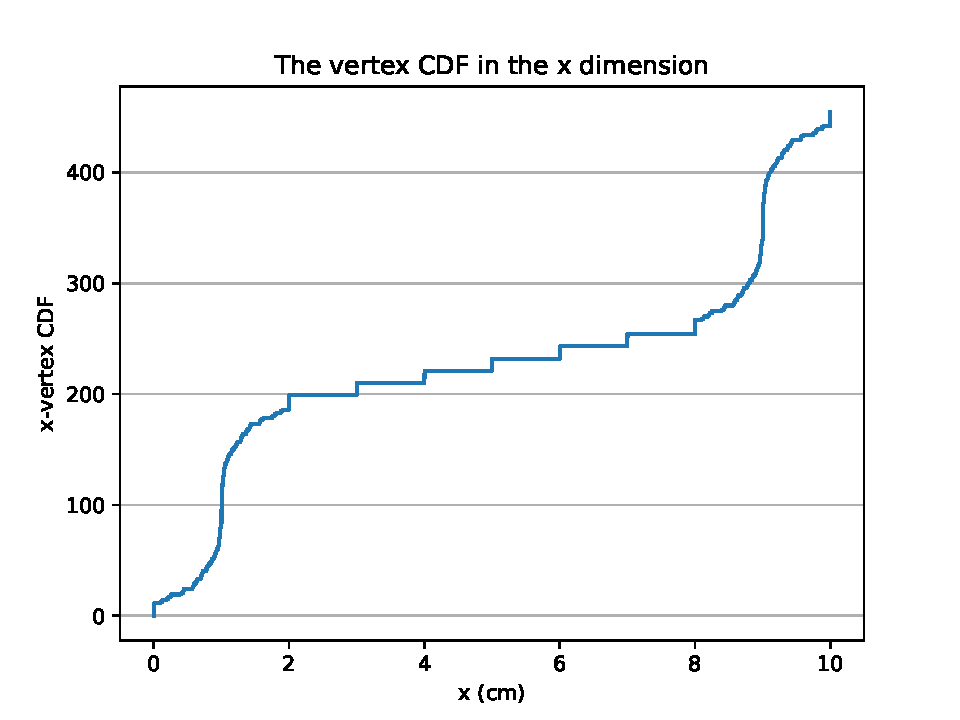
\includegraphics[scale=0.75]{../figures/xvertexcdf.pdf}
\caption{The x-vertex CDF of the mesh shown in Fig.~\ref{natural_boundary_example}}.
\label{vert_cdf}
\end{figure}

To identify where the jumps in the CDF occur, we take the derivative of the CDF and isolate the largest discontinuities in it. Figure~\ref{gradcdf} plots the derivative of the CDF shown in Fig.~\ref{vert_cdf}.
\begin{figure}[h]
\centering
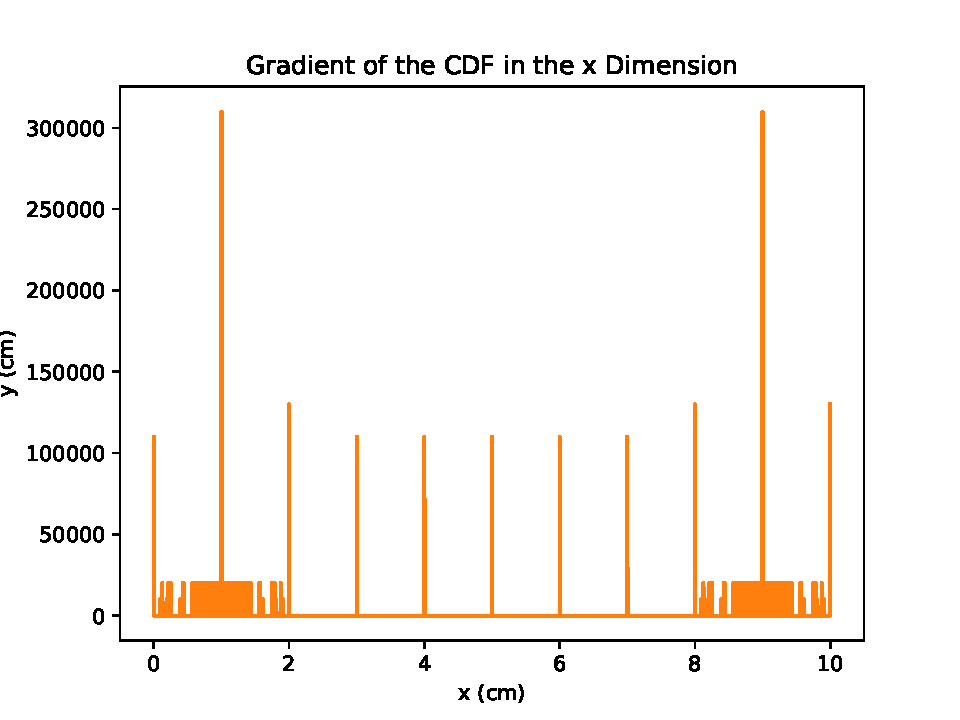
\includegraphics[scale=0.75]{../figures/gradcdf.pdf}
\caption{The derivative of the CDF shown in Fig.~\ref{vert_cdf}}.
\label{gradcdf}
\end{figure}
The largest discontinuities in Fig.~\ref{gradcdf} occur at the instances where there are natural boundaries all the way through the mesh, or at 1 cm intervals.
We should note that although the global boundaries of the problem have discontinuities, these discontinuities are obviously not eligible to be chosen as optimized partitions.

\FloatBarrier
\subsection{Finding Natural Boundaries for Sets of Columns}
In order to globalize the optimization of the cut lines per column, we set up a binary tree of test cases, such as the one shown in Fig.~\ref{binary_tree}. Each layer in the tree represents one set of $y$ cut lines. The first layer, or the root of the tree, represents the case where we try and find the natural boundaries in $y$ throughout all columns, in this case 4 columns. The next layer tries to find two sets of natural boundaries, one set of natural $y$ boundaries through the first two columns, and another set through the final 2 columns. Finally, the last case finds a set of natural $y$ boundaries in each individual column.

\begin{figure}[h]
\centering
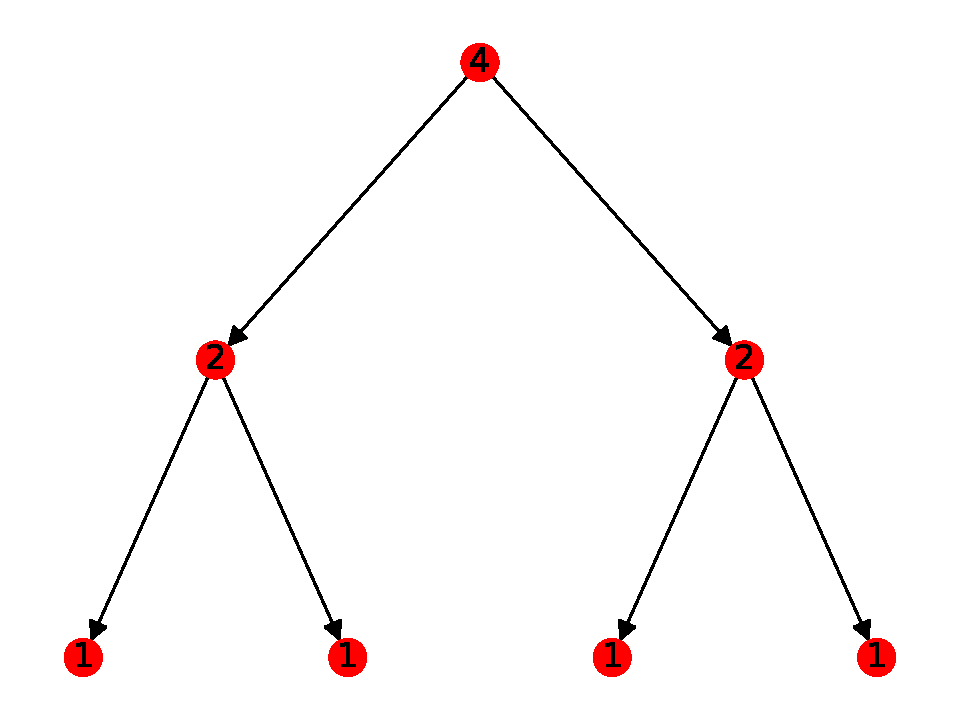
\includegraphics[scale=0.75]{../figures/binary_tree.pdf}
\caption{A binary tree where each node represents the number of columns we are attempting to find a natural boundary through.}
\label{binary_tree}
\end{figure}
\jcr{make sure the arrow tips are LARGE enough to see}

Let's\jcr{no abbreviations please} consider the mesh of the Level 2 \jcr{hyphen this throughout: Level-2} experiment shown in Fig.~\ref{level2_nocut}.
We run this problem with 42 subsets in $x$ and 13 subsets in $y$.
Fig.~\ref{opt_walkthrough} shows 3 stages of choosing partitions for the Level 2 mesh.
Fig.~\ref{42} shows the $x$ partitions, with the $y$ partitions optimized for all 42 columns.
This means that we attempted to identify natural boundaries through all 42 columns.
Fig.~\ref{21} shows the same $x$ partitions, but the $y$ partitions optimized for the first 21 columns independently from the second 21 columns.
Fig.~\ref{10} shows the same $x$ partitions, with the $y$ partitions optimized independently for first 10 columns, then the next 11 columns, then the next 10 columns, then the next 11 columns.
We continue this process until we are optimizing $y$ partitions for each column.
%%%%%%%%%%%%%%%
\begin{figure}[h]
\centering
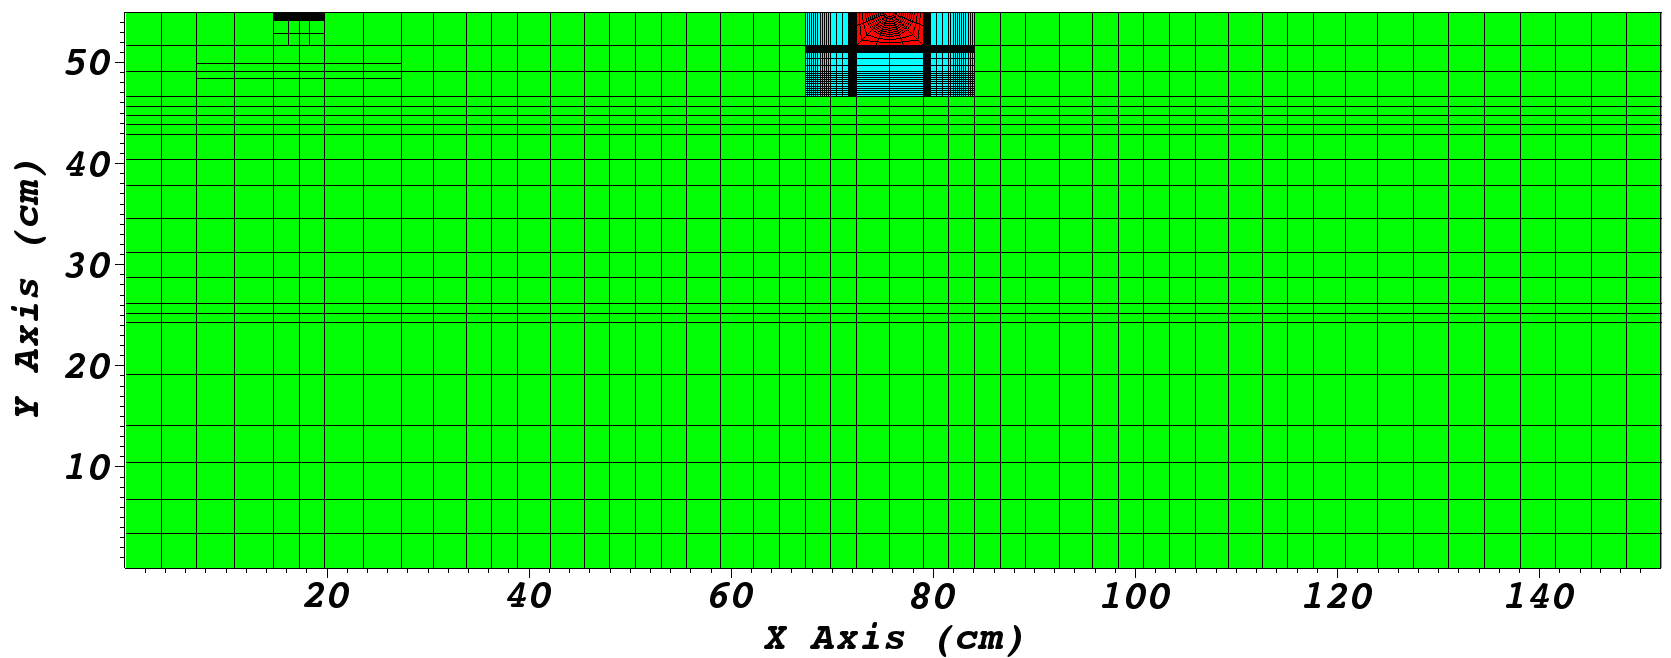
\includegraphics[scale=0.3]{../../figures/level2_nocut.png}
\caption{The mesh for the Level 2 experiment.}
\label{level2_nocut}
\end{figure}

\begin{figure}[h]
\centering
  \begin{subfigure}[t]{\textwidth}
    \centering
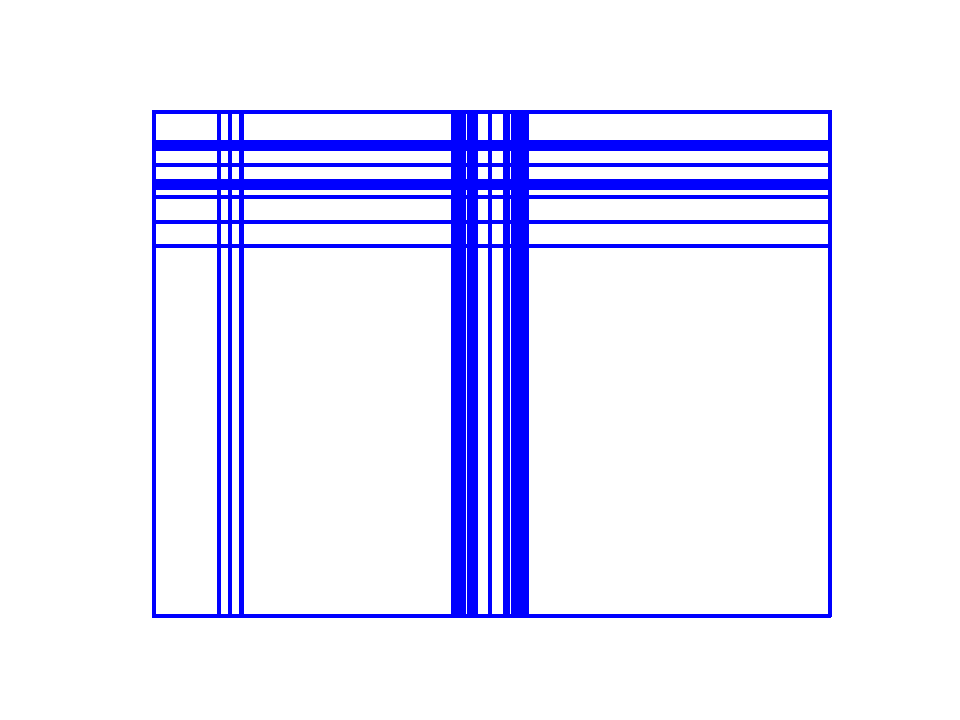
\includegraphics[scale=0.5]{../../figures/lvl2_suite_0.pdf}
  \caption{The y-cuts chosen for all 42 columns.}
    \label{42}
  \end{subfigure}
  \begin{subfigure}[b]{\textwidth}
    \centering
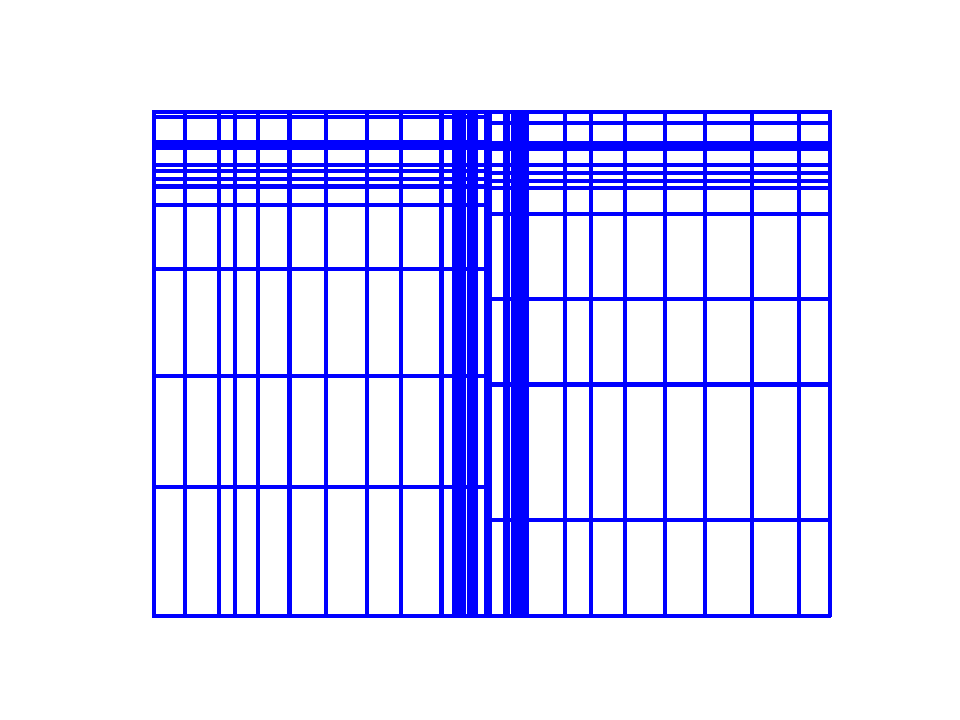
\includegraphics[scale=0.5]{../../figures/lvl2_suite_1.pdf}
    \caption{The y-cuts chosen independently for the first 21 columns and the second 21 columns}.
    \label{21}
  \end{subfigure}
  \begin{subfigure}[b]{\textwidth}
    \centering
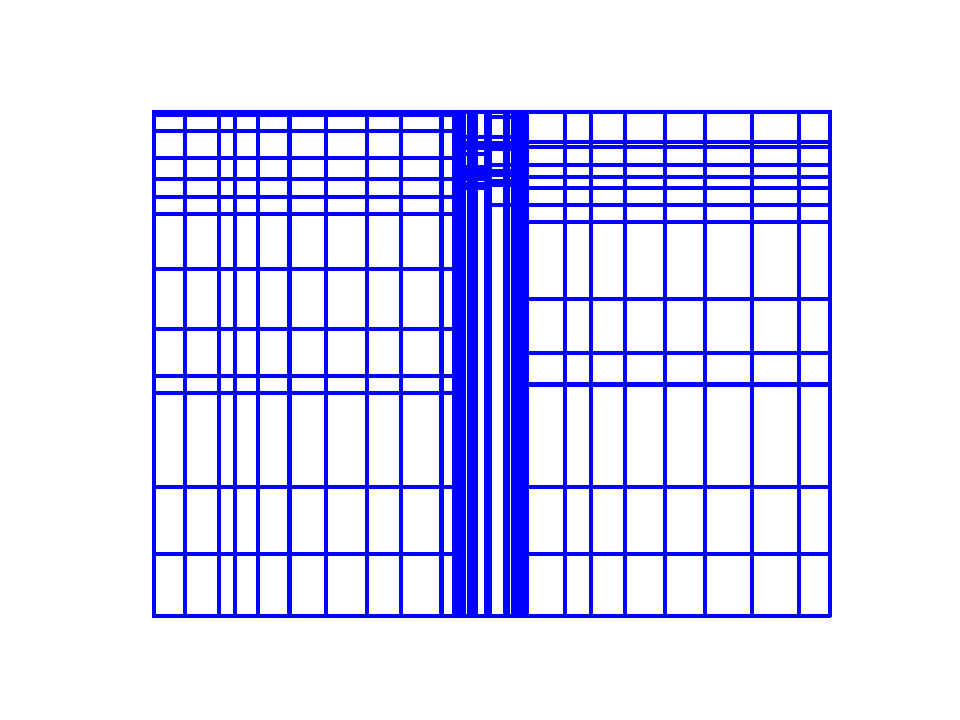
\includegraphics[scale=0.5]{../../figures/lvl2_suite_2.pdf}
    \caption{The y-cuts chosen for independently for 10,11,10, and 11 columns.}
    \label{10}
  \end{subfigure}
  \caption{The Level 2 Mesh partitions at three stages of the choosing the optimization cut process.}
  \label{opt_walkthrough}
\end{figure}

This method of optimization allows us to select a set of partitions with an attempt to optimize over the global domain.
With this method, we are also not running the time-to-solution estimator a large number of times, instead electing to using\jcr{use it in} an intuitive automation process.

\FloatBarrier

\section{Optimization Results}
The CDF optimization method was run on the unbalanced pin mesh and the Level 2 experiment mesh.
The unbalanced pin mesh was run through the optimization suite from 2 to 10 subsets in each dimension.
Figure~\ref{ubp_opt} shows the time-to-solution for optimized, regular, load-balanced and load-balanced-by-dimension cuts on the unbalanced pins mesh from 2 to 10 subsets in each dimension.
%%%%%%%%%%
\begin{figure}[ht]
\centering
  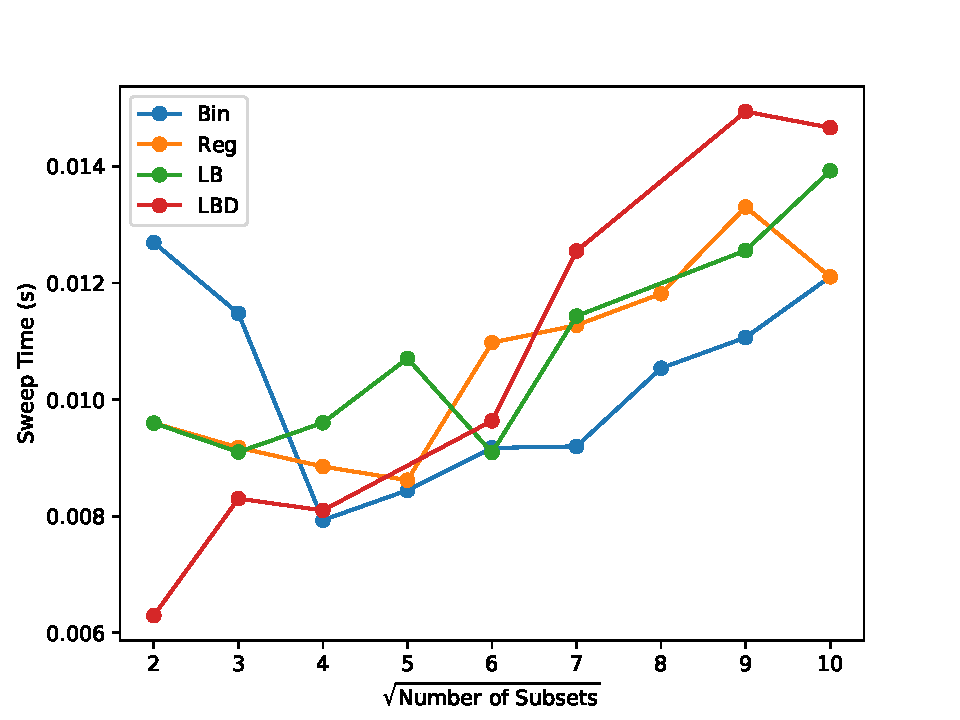
\includegraphics{../../figures/unbalanced_pins_opt_comparison.pdf}
  \caption{The time-to-solution for optimized, regular, load-balanced and load-balanced-by-dimension cuts on the unbalanced pins mesh from 2 to 10 subsets in each dimension.}
  \label{ubp_opt}
\end{figure}
%%%%%%%%%%%
For low numbers of subsets, the load-balanced-by-dimension partitions outperform the regular, load-balanced, and optimized partitions.
Due to the low number of communications, having partitions that are balanced by column doesn't incur a large communication penalty, and having a well-balanced problem is still more important.
However, once we exceed 16 subsets, we can see the optimized partitions outperforming the other partition types, with the prioritization of not adding cells paying off.

Figure~\ref{level2_opt} shows the sweep times on the Level 2 mesh from the time-to-solution estimator and PDT for (1) regular cuts, (2) hand-balanced cuts, (3) load-balanced cuts, (4) load-balanced-by-dimension cuts, and (5) optimized cuts.
\begin{figure}[H]
\centering
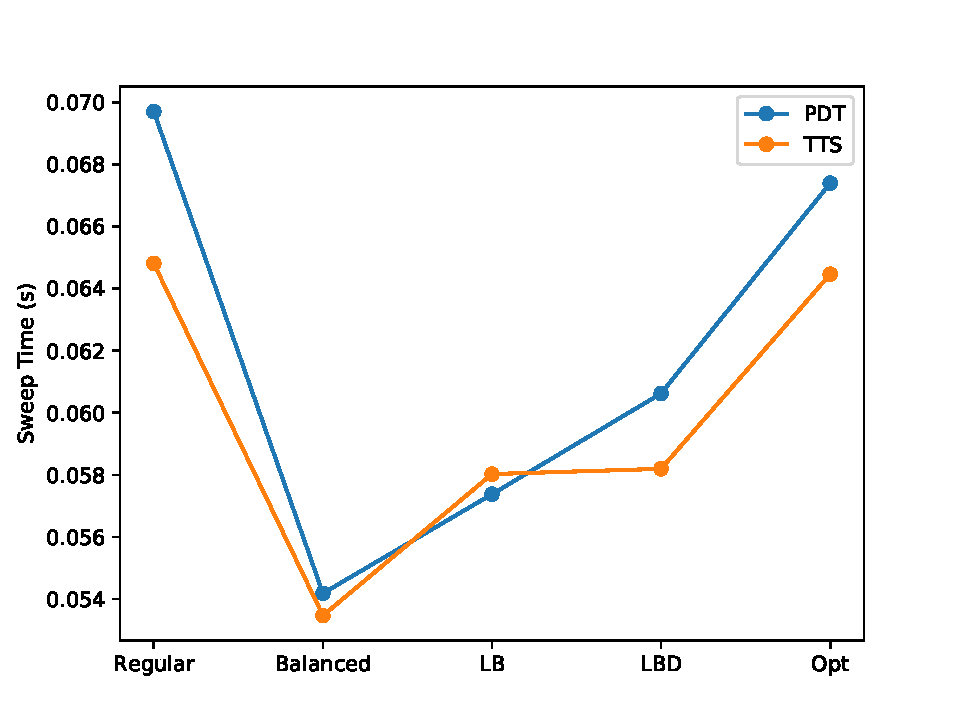
\includegraphics{../../figures/level2_sweep_comp.pdf}
\caption{The Level 2 mesh sweep times from the time-to-solution estimator and PDT for (1) regular cuts, (2) hand-balanced cuts, (3) load-balanced cuts, (4) load-balanced-by-dimension cuts, and (5) optimized cuts. }
\label{level2_opt}
\end{figure}
This problem shows us\jcr{remove us. This is written English. Take the time before writing down something. The opportunities for me to come after you and check are now very limited. Make sure that what you have added to tip top} that this optimization approach will at times not give us the best sweep times.
While prioritizing not adding cells to the mesh is a sensible argument, sometimes adding cells to achieve better balance may pay off.
The importance of making sure to run the regular, load-balanced, and load-balanced-by-dimension cuts in addition to the optimized cuts is made clear by this problem.
Thus the ``optimization suite'' should always have the cut types of previous work to test.
In addition, spending the time to hand balance the mesh is potentially not worth it as the time per sweep only differed by 0.004 seconds.
Depending on the total number of sweeps that need to be performed, this difference could be negligible in the total time to solution.

The failure of the optimization process to provide better cuts for the Level 2 experiment highlights a few paths forward for future work.
The time-to-solution estimator is computationally too slow (the Level 2 problem takes 20 seconds per run) to run a large number of partition sets.
With a faster time-to-solution estimator (down to milliseconds for modestly large problems), we could  run a much larger number of partitions to test their time-to-solution in a reasonable time, and our optimization process could be more robust.
Combinations of natural boundaries could be selected instead of just the highest discontinuities in the CDF.
For example, choosing 42 of the largest 50 cuts in the $x$ direction for the Level-2 problem alone would give us 14,190 potential cuts to try in just the $x$-direction.
At 20 seconds per run, this would take approximately 79 hours, which is unfeasible.
However, at 20 milliseconds per run, this would only take around 5 minutes, which is a reasonable amount of time to wait for optimized partitions.
